% Clase de documento (Utilizar la que interese)
\documentclass{scrbook}

%%%%%%%%%%%%%%%%%%%%%%%%%% REMARK %%%%%%%%%%%%%%%%%%%%%%%%%% 
\newif\ifremark
\long\def\remark#1{
\ifremark%
        \begingroup%
        \dimen0=\columnwidth
        \advance\dimen0 by -1in%
        \setbox0=\hbox{\parbox[b]{\dimen0}{\protect\em #1}}
        \dimen1=\ht0\advance\dimen1 by 2pt%
        \dimen2=\dp0\advance\dimen2 by 2pt%
        \vskip 0.25pt%
        \hbox to \columnwidth{%
                \vrule height\dimen1 width 3pt depth\dimen2%
                \hss\copy0\hss%
                \vrule height\dimen1 width 3pt depth\dimen2%
        }%
        \endgroup%
\fi}
\remarktrue

% MÁRGENES DE LAS PÁGINAS
\usepackage[
  inner	=	3.0cm, % Margen interior
  outer	=	2.5cm, % Margen exterior
  top	=	2.5cm, % Margen superior
  bottom=	2.5cm, % Margen inferior
  includeheadfoot, % Incluye cabecera y pie de página en los márgenes
]{geometry}
\usepackage{hyperref}
\hypersetup{ colorlinks=true, urlcolor=red }
% Valor de interlineado
\renewcommand{\baselinestretch}{1.2} % 1.2 línea de interlineado

% Paquetes imprescindibles para la portada
\usepackage{fontspec} % Para poder importar las fuentes
\usepackage{textpos} % Para posicionar bloques de texto
\usepackage{graphicx} % Para cargar imágenes
\usepackage{setspace} % Para modificar los espacios arriba y abajo
\usepackage{minted}
\usepackage{pdfpages}


% Universidad y facultad
\newcommand{\Universidad}{Universitat Politècnica de València}
\newcommand{\LogoUniversidad}{logos-universidad/LogoUPV}
\newcommand{\Facultad}{Departamento de Informática de Sistemas y Computadores}
\newcommand{\LogoFacultad}{logos-universidad/logo-etsinf}
% Titulación
\newcommand{\Titulacion}{Máster en Ingeniería de computadores y redes}
% Título del trabajo
\newcommand{\titulo}{Interfaz MQTT para la API Web de Open Weather Map}
% Tipo de trabajo
\newcommand{\tipotrabajo}{Trabajo final Sistemas basados en Redes Móviles}
% Datos del autor
\newcommand{\miNombre}{Miguel Antonio Avargues Gutiérrez}
% Ubicación
\newcommand{\miUbicacion}{València}


\begin{document}


%%%%% PORTADA
%%%%%%%%%%%%%%%%%%%%%%%%%%%%%%%%%%%%%%%%%%%%%%%%%%%%%%%%%%%%%%%%%%%%%%%%
% Plantilla TFG/TFM
% Realizado por: Jose Manuel Requena Plens
% Contacto: info@jmrplens.com / Telegram:@jmrplens
%%%%%%%%%%%%%%%%%%%%%%%%%%%%%%%%%%%%%%%%%%%%%%%%%%%%%%%%%%%%%%%%%%%%%%%%

% Fuentes
\newfontfamily\ArialMT{ArialMT}[Path=./fuentes/] 
\newfontfamily\ArialBoldMT{Arial-BoldMT}[Path=./fuentes/] 
\newfontfamily\ArialBoldItalicMT{Arial-BoldItalicMT}[Path=./fuentes/] 

\begin{titlepage}

% Márgenes de esta pagina modificados
\newgeometry{ignoreall,top=2.5cm,bottom=1cm,outer=2.5cm,inner=2.5cm}

% Pagina sin estilo
\thispagestyle{empty}

%%%%%%%%%%%%%%%%%%%%%%%%%%%%%%%%%%%%%%%%%%
% Universidad, facultad y titulación
\noindent\begin{minipage}{\textwidth}
\centering
% Universidad
 {\ArialMT\fontsize{20pt}{25pt}
 {\addfontfeature{LetterSpace=1.0}
 {\MakeUppercase\Universidad}}}\\[0.5cm]
% Facultad
 {\ArialBoldMT\fontsize{14pt}{17pt}
 {\addfontfeature{LetterSpace=10.0}{
 \MakeUppercase\Facultad}}}\\[0.42cm] 
% Titulación
 {\ArialBoldMT\fontsize{13pt}{16pt}
 {\addfontfeature{LetterSpace=16.0}{
 \Titulacion}}}
\noindent\rule[-0.22cm]{\textwidth}{5pt} % Linea
\end{minipage}

% Relleno hasta logotipos
\vfill

%%%%%%%%%%%%%%%%%%%%%%%%%%%%%%%%%%%%%%%%%%
% Logotipos
% Universidad
\begin{textblock*}{4cm}(1.45cm,-6.52cm)% Ancho - Pos X,PosY
	 \includegraphics[width=4cm]{\LogoUniversidad}
\end{textblock*}
% Facultad
\begin{textblock*}{10cm}(8cm,-5.82cm)% Ancho - Pos X,PosY
	 \includegraphics[width=6cm]{\LogoFacultad}
\end{textblock*}

% Relleno hasta el título
\vfill

%%%%%%%%%%%%%%%%%%%%%%%%%%%%%%%%%%%%%%%%%%
% Título
\begin{textblock*}{\textwidth}(0cm,-6.1cm)% Ancho - Pos X,PosY
\noindent
\begin{minipage}{\textwidth}
\begin{spacing}{2.1}
 \centering
  {\fontsize{25pt}{30pt}\ArialBoldMT
  {\addfontfeature{}
 \titulo}}
\end{spacing}
\end{minipage}
\end{textblock*}

% Relleno hasta autor y tutores
\vfill

%%%%%%%%%%%%%%%%%%%%%%%%%%%%%%%%%%%%%%%%%%
% Tipo, Autor y Tutores
\begin{textblock*}{7.35cm}(8.65cm,-7.88cm)% Ancho - Pos X,PosY
\begin{flushleft}
% Tipo trabajo
 {\ArialBoldItalicMT\fontsize{12pt}{14pt}
 {\addfontfeature{}
 {\MakeUppercase\tipotrabajo}}}\\[0.49cm]
% Autor
 {\ArialMT\fontsize{12pt}{14pt}
 {\addfontfeature{}
 Autor:}}\\ 
 {\ArialBoldMT\fontsize{12pt}{14pt}
 {\addfontfeature{}
 {\miNombre}}}\\[0.5cm]
% Tutores
% {\ArialMT\fontsize{12pt}{14pt}
% {\addfontfeature{}
% Tutor/a:}}\\
% {\ArialBoldMT\fontsize{12pt}{14pt}
% {\addfontfeature{}
% {\miTutor}}}\\[0.49cm]
% Localidad y Fecha
 {\ArialBoldItalicMT\fontsize{12pt}{14pt}
 {\addfontfeature{}
 {\MakeUppercase \miUbicacion, \number\year}}}
\end{flushleft}
\end{textblock*}



\end{titlepage} % Fin de portada

% A partir de aquí aplica los márgenes establecidos en configuracioninicial.tex
\restoregeometry


 % Portada B/N

%%%%% RESUMEN
%%%%%%%%%%%%%%%%%%%%%%%%%%%%%%%%%%%%%%%%%%%%%%%%%%%%%%%%%%%%%%%%%%%%%%%%
% Plantilla TFG/TFM
% Realizado por: Jose Manuel Requena Plens
% Contacto: info@jmrplens.com / Telegram:@jmrplens
%%%%%%%%%%%%%%%%%%%%%%%%%%%%%%%%%%%%%%%%%%%%%%%%%%%%%%%%%%%%%%%%%%%%%%%%
\thispagestyle{empty}
%\section*{Abstract}

%Resumen en inglés.

%\paragraph*{Keywords}

%Palabras; Clave; Del; Trabajo; En; Inglés;

\section*{Resumen}

En este documento se describen los pasos realizados para implementar una interfaz Python mediante el uso del protocolo MQTT para la API web de la página \href{http://openweathermap.org/}{Open Weather Map} (ver \url{http://openweathermap.org/}). También los pasos necesarios para realizar un despliegue en un servicio \textit{cloud} (en este caso, Amazon Web Services). Se anexa el código de la interfaz web.

\paragraph*{Palabras clave}

MQTT; Open; Weather; Map; Openweathermap; Python; API;

%%%%% INDICES
\tableofcontents

%%%%% Resto del documento
\chapter{Introducción}
\section{Descripción del problema}
En la edad actual de la información, el intercambio de esta es clave. En internet, se pueden dar diversas formas de realizar este intercambio. Uno de los protocolos más utilizados debido a ser la forma clave de realizar la transmisión de páginas web es el protocolo de transferencia de hipertexto - Hypertext Transfer Protocol en inglés y comúnmente referido simplemente como HTTP -

Aunque este es el estándar para la transferencia de páginas web, su uso no se limita únicamente a la transmisión de estas. La arquitectura de Transferencia de Estado Representacional - Representational State Transfer en inglés o REST - define el uso de algunas de las peticiones deifnidas en el protocolo HTTP con tal de ofrecer una interfaz capaz de crear, leer, modificar y eliminar datos de algún recurso controlador por un servidor Web. Un ejemplo sería la interfaz web ofrecida por \href{http://openweathermap.org/}{Open Weather Map (OWM)} con tal de obtener información relativa a la meteorología y datos similares.

Pese a ser muy flexible HTTP no es la única forma de transmitir datos entre dos máquinas (conocido como comunicación machine-to-machine o m2m). Otras alternativas son <<Cap'n Proto>>, <<SOAP>> o <<MQTT>>. En este trabajo nos vamos a centrar en <<MQTT>>, un protocolo basado en mensajes que necesita de un servidor (que puede ser replicado o funcionar al mismo tiempo con varios) conocido como \textit{broker}, con tal de direccionar los mensajes desde el publicador (cliente o nodo que genera los datos) hasta el suscriptor (cliente o nodo que utiliza los datos). Además, ofrece otras ventajas como por ejemplo la asincronía de mensajes o el envío de mensajes a todos los clientes que se suscriban al mismo \textit{topic}, que podría verse como un buzón de mensajes compartidos en el cual cada nodo decide si apuntarse o no.

\section{Objetivos}
\label{cap:objetivos}
En este proyecto se va a realizar un pequeño programa Python con tal de poder realizar llamadas a la API REST ofrecida por \href{http://openweathermap.org/}{Open Weather Map} mediante mensajes MQTT. También los pasos necesarios para desplegar esta interfaz MQTT a REST (IMR) así como un servidor <<Mosquitto>> (el \textit{broker}) en una instancia de un proveedor \textit{cloud} (Amazon Web Services para ser precisos). Para ello se definen los siguientes pasos:

\begin{itemize}
    \item Definir una arquitectura de la comunicación.
    \item Realizar la implementación del programa Python.
    \item Desplegar la aplicación y el servidor en el proveedor \textit{cloud}.
\end{itemize}

Este trabajo se realiza de forma principalmente práctica y por ello va a estar organizado como un tutorial con tal de conseguir los objetivos planteados.

\section{Estructura del documento}
Para alcanzar los objetivos mencionados, esta memoria se ha estructurado en cinco capítulos:

\begin{itemize}
    \item En el capítulo \ref{cap:arquitectura} se comenta la arquitectura diseñada para la interacción. Se muestran los componentes y se expone la forma en la que se comunican entre ellos. 
    \item El capítulo \ref{cap:implementación} presenta los detalles sobre la implementación de la interfaz. Se realiza un estudio breve del nivel gratuito de la interfaz de OWM, cómo se consigue la clave para utilizar la API REST y los detalles de la implementación de la IMR.
    \item El capítulo \ref{cap:despliegue_cloud} describe paso a paso la forma en la que se puede realizar un despliegue del sistema desarrollado (servidor MQTT + interfaz) en un proveedor de servicios \textit{cloud}.
    \item Finalmente, en el capítulo \ref{cap:conclusiones} se comentan los objetivos alcanzados de los que se han propuesto en \ref{cap:objetivos}. Para concluir, se comenta futuro trabajo a realizar.
\end{itemize}

\chapter{Arquitectura del sistema}
\label{cap:arquitectura}

La arquitectura propuesta para la interfaz se puede observar en la figura \ref{fig:arquitectura_comm}. Como se puede observar en esta, se espera que la interfaz sea capaz de dar servicio a diversos usuarios al mismo tiempo. Aunque esta no haga uso de varios hilos el \textit{broker} ofrecerá las peticiones de una en una, haciendo que la interfaz pueda hacer frente a posibles picos de carga.

\begin{figure}[tbh] 
\begin{center}
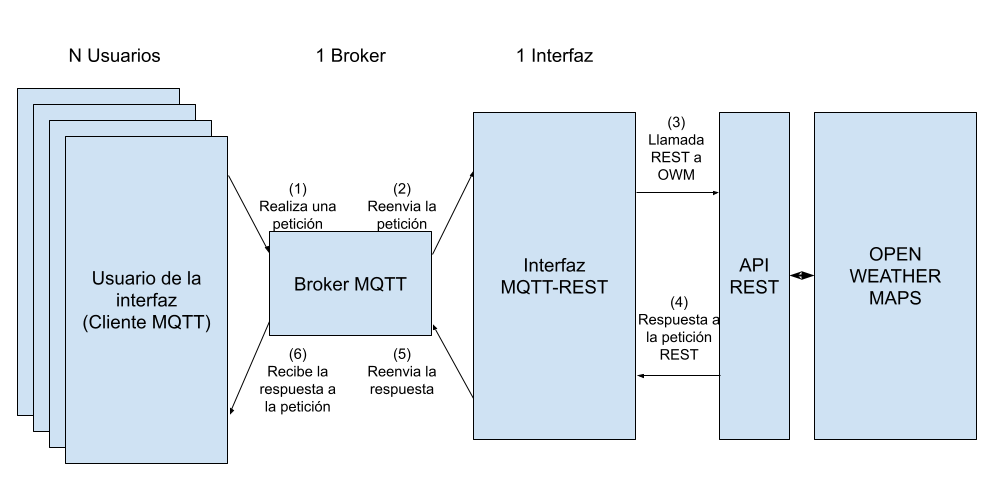
\includegraphics[width=1\textwidth]{figuras/arquitectura_comm.png}
\caption{Modelo de la comunicación desde que el usuario realiza una llamada hasta que obtiene la respuesta.} 
\label{fig:arquitectura_comm}
\end{center}
\end{figure}

Las peticiones seguirán el ciclo de vida mostrado en la figura anteriormente mencionada, a continuación se entra en algo más de detalle sobre este ciclo de vida.

\begin{enumerate}
    \item El usuario de la interfaz realiza una llamada bajo una estructura predefinida de mensaje (más información en el capítulo \ref{cap:implementación}). Esta llega al \textit{broker}.
    \item El \textit{broker} se encarga de reenviar la petición a la IMR.
    \item La IMR interpreta los parámetros del mensaje MQTT, transformándolos en una llamada al \textit{endpoint} correspondiente de la API REST de Open Weather Maps.
    \item La IMR recibe la respuesta a la petición que ha conseguido y la empaqueta en un mensaje MQTT.
    \item La IMR envía la respuesta empaquetada al \textit{broker}. 
    \item El \textit{broker} avisa al usuario de que ha recibido una respuesta y se la envía para que pueda utilizar los datos que pidió.
\end{enumerate}


\chapter{Implementación del programa}
\label{cap:implementación}

En las siguientes secciones se detallan los pasos seguidos con tal de desarrollar la interfaz. Para ello se va a describir brevemente el funcionamiento de la API REST OWM. Tras ello cómo obtener la clave para poder realizar llamadas a la API. Finalmente se discuten los detalles más importantes de la implementación de la interfaz.

\section{Estudio de la API de OWM}
Open Weather Map ofrece distintos niveles para utilizar su interfaz bajo un servicio de pago mensual. En la realización de este trabajo se ha utilizado el nivel gratuito, que  ofrece 1000000 de llamadas gratuitas mensuales para obtener datos del tiempo atmosférico actual, así como de contaminación del aire y \textit{Geocoding}. Además, ofrece 1000 llamadas a la interfaz <<One Call API>>, capaz de obtener tiempo atmosférico actual, previsión de la próxima hora por minutos, previsión de los próximos dos días por hora, previsión de la próxima semana día a día, alertas meteorológicas nacionales y el histórico de los últimos cinco días.

El conjunto de todas estas APIs se pueden resumir en cuatro destinos diferentes para las peticiones, una por servicio.
\begin{enumerate}
    \item Para las peticiones del tiempo actual: https://api.openweathermap.org/data/2.5/weather
    \item En caso de querer realizar una llamada a la interfaz <<One Call>>:\\ https://api.openweathermap.org/data/2.5/onecall
    \item Las peticiones de contaminación del aire utilizan el destino: http://api.openweathermap.org/\\data/2.5/air\_pollution
    \item Si se desea utilizar el servicio de \textit{geocoding}: http://api.openweathermap.org/geo/1.0/
\end{enumerate}

La interfaz MQTT-REST deberá ofrecer la posibilidad de realizar una llamada a cualquiera de estos cuatro \textit{endpoints}. Además, deberá permitir el uso de cualquier llamada a un \textit{sub-endpoint}, por ejemplo, realizar una llamada \textit{geocoding} directa (cuyo destino es\\ http://api.openweathermap.org/geo/1.0/direct) o inversa (http://api.openweathermap.org/\\geo/1.0/reverse).

\section{Obtención de la clave API}
Antes de poder desarrollar la aplicación, es necesario obtener la clave API con tal de poder obtener respuesta a las llamadas que se hagan a OWM. Por ello hay que registrarse previamente, una vez se haya completado el registro y confirmado la dirección de correo electrónico existen dos formas de obtener la clave para acceder a la API:\footnote{Las claves que se muestran en las figuras difieren porque son de dos cuentas diferentes, si son de la misma cuenta es la misma clave tanto en el correo como en la página web.}

\begin{itemize}
    \item En un correo que nos envia OWM (figura \ref{fig:api_correo})
    \item En la página "API Keys" de \href{http://openweathermap.org/api_keys}{Open Weather Map} (figura \ref{fig:api_web})
\end{itemize}

\begin{figure}[tbh] 
\begin{center}
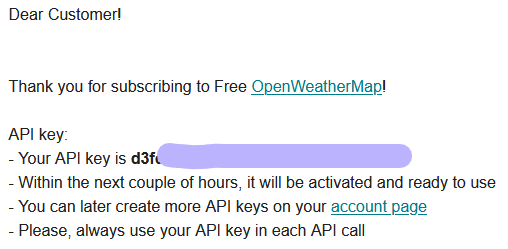
\includegraphics[width=1\textwidth]{figuras/api_correo.png}
\caption{Fragmento del correo con la clave de acceso a la API.} 
\label{fig:api_correo}
\end{center}
\end{figure}

\begin{figure}[tbh] 
\begin{center}
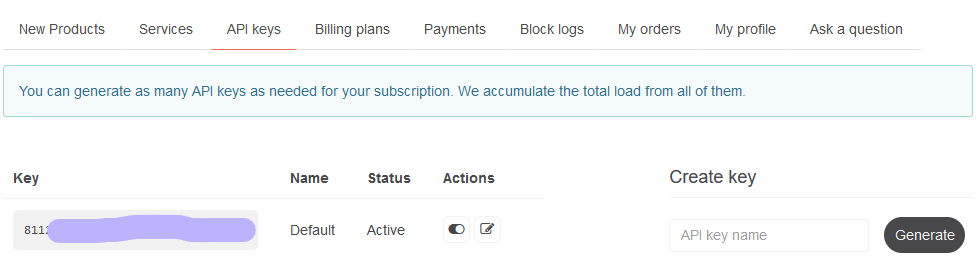
\includegraphics[width=1\textwidth]{figuras/api_web.png}
\caption{Página web con la clave de acceso a la API.} 
\label{fig:api_web}
\end{center}
\end{figure}

\section{Implementación en Python}
Para la implementación de la interfaz se han utilizado los siguiente paquetes:

\begin{itemize}
    \item "requests": se encarga de realizar las llamadas HTTP a los diferentes \textit{endpoints}.
    \item "json": se encarga de convertir e interpretar mensajes desde/a formato JSON.
    \item "paho.mqtt.client": libreria que ofrece el soporte a nivel de cliente para MQTT. Con esta libreria somos capaces de conectarnos al \textit{broker} con tal de poder enviar y recibir mensajes.
    \item "time": utilizada principalmente para gestionar las peticiones que se pueden realizar por minuto para los diferentes tipos de API.
\end{itemize}

El funcionamiento de la interfaz es muy sencillo. Primero intenta conectarse con el servidor definido en la variable "MQTT\_SERVER" en el puerto "MQTT\_PORT". Si la conexión tiene éxito, se ejecuta la función "on\_connect", donde se suscribe al \textit{topic} "help" (línea 37) y a cualquier \textit{topic} hijo de "reqs" (l. 36).

Cuando recibe un mensaje desde el \textit{topic} "help", simplemente envía un mensaje al mismo \textit{topic} con un pequeño texto de ayuda (l. 428). En caso de recibir un mensaje por otro \textit{topic} (solo puede ser desde un \textit{topic} hijo de "reqs"). Intenta interpretar el mensaje JSON. Este mensaje tiene una estructura variable, pero debe contener, como mínimo dos parámetros:

\begin{itemize}
    \item "CallType": describe que \textit{endpoint} utilizar, se distingue entre "CurrentWeather", "OneTime", "AirPollution" y "Geocoding".
    \item "type": permite saber qué tipo de llamada se va a realizar al \textit{endpoint}, por ejemplo en el caso de realizar una llamada para conocer el tiempo atmosférico actual (en la que "CallType" == "CurrentWeather") se distingue entre llamada con el nombre de la ciudad ("type" == "city"), por identificador de la ciudad ("type" == "id"), por geocoordenadas  ("type" == "geo") o por código postal  ("type" == "zip"). Cada \textit{endpoint} tiene diferentes "type" que coincide con las diferentes llamadas que se pueden realizar sobre ese \textit{endpoint}.
\end{itemize}

Además, cada "type" de llamada diferente tiene sus parámetros necesarios (por ejemplo, siguiendo el ejemplo anterior de una llamada para conocer el tiempo actual pero con "type" == "geo", la latitud y longitud son necesarios para saber de qué lugar se quieren obtener los datos) y opcionales (suelen ser compartidos para cada \textit{endpoint}, por ejemplo, las unidades en las que retornar la información, el idioma o el formato de respuesta\footnote{Para más información sobre los posibles parámetros, ver la documentación en el anexo \ref{anexo:IMR-docs} o en \href{http://shorturl.at/akyES}{este enlace}}).

Una vez la interfaz ha interpretado todos los parámetros presentes de la llamada, que ha recibido en el mensaje empaquetado como JSON, esta realiza la llamada al \textit{endpoint} correspondiente mediante el paquete "requests". Una vez llegado a este punto, aunque la respuesta que OWM ofrece no sea correcta la interfaz simplemente la retransmitirá como resultado en el \textit{sub-topic} "resp" del \textit{topic} donde se recibió el mensaje, ya que la llamada se ha realizado con éxito (aunque la respuesta haya sido un error).\footnote{Aunque el formato de respuesta sea diferente a JSON, la interfaz siempre devolverá los datos empaquetados en un mensaje JSON, dentro del campo "res" del payload. Los datos extraídos de esta variable estarán en el formato deseado (JSON, XML o HTML).} Mencionar que si existe algún error en el formato del mensaje (por ejemplo faltan parámetros necesarios), la interfaz avisa mediante un mensaje en el \textit{sub-topic} "resp" (como una respuesta normal).

Al acabar la interfaz se realizó un pequeño documento en "Google Drive" a modo de documentación para el usuario. En este se detalla el uso básico de la API, la estructura de los mensajes y todos los posibles parámetros (tanto necesarios como opcionales) para cada tipo de petición que se soporta. También ofrece el nombre del host al que conectarse para poder utilizar la interfaz.

Con tal de respetar los límites máximos del nivel gratuito de OWM. La interfaz está limitada a 23 mensajes por minuto para consultas del tiempo actual, \textit{geocoding} y contaminación del aire. Por otra parte, se puede realizar una llamada a la interfaz "One Call" una vez cada minuto y medio. De esta forma se llega a casi el máximo de peticiones mensuales.

Todo el código desarrollado se puede observar en el anexo \ref{anexo:codigo_interfaz}. La documentación para el uso de la IMR se puede ver en \href{http://shorturl.at/akyES}{este enlace} o en el anexo \ref{anexo:IMR-docs}.

\chapter{Despliegue en la nube}
\label{cap:despliegue_cloud}

Este capítulo contiene todos los pasos para el despliegue del servicio (servidor MQTT + IMR) en la infraestructura \textit{cloud} de Amazon. Se define como crear la instancia virtual gratuita, cómo instalar el servidor mosquitto, como iniciar la IMR y como crear un (sencillo) supervisor del servidor mosquitto.

\section{Creación de la instancia}
Se supone acceso a una cuenta y en la página de inicio.
\begin{enumerate}
    \item En la barra de búsqueda de servicios introducir "EC2" (figura \ref{fig:paso1-ec2}).
    \item Seleccionar la opción "Lanzar instancias" en la esquina superior derecha (figura \ref{fig:paso2-ec2}).
    \item Como sistema operativo, se elige "Ubuntu Server 20.04 LTS". Click en "Seleccionar" (figura \ref{fig:paso3-ec2})
    \item A continuación se pide seleccionar el tipo de instancia. Cualquiera sería válida, en este trabajo se ha utilizado la instancia t2.micro ya que AWS ofrece un año de prueba sin coste. Se podrían elegir otras instancias y realizar un pago por uso. Click en "Sigueinte: Página Configuración de los detalles de la instancia" (figura \ref{fig:paso4-ec2}).
    \item En el selector de pasos en la parte superior, elegir "Página Configure Security Group" (figura \ref{fig:paso5-ec2}).
    \item Crear todas las reglas necesarias para que el puerto 1883 UDP y TCP en IPv4 así como IPv6 estén disponibles desde "cualquier lugar". También se puede abrir el puerto 80 TCP y UDP por si acaso (aunque no se realiza un uso directo de este, podría llegar a dar problemas con la API REST de OWM). Click en "Revisar y Lanzar" (figura \ref{fig:paso6-ec2}).
    \item Click en "Lanzar" (figura \ref{fig:paso7-ec2}).
    \item Nos pedirá crear un par nuevo de claves, al cual habrá de nombrar y seguidamente descargar para poder acceder posteriormente a la instancia mediante SSH. Tras nombrar el par de claves click en "Descargar par de claves" \textbf{es muy importante el descargar las claves y tener una copia del fichero siempre en un lugar conocido} y tras ello "Lanzar instancias" (figura \ref{fig:paso10-ec2}).
\end{enumerate}

\begin{figure}[htb] 
\begin{center}
\label{fig:paso1-ec2}
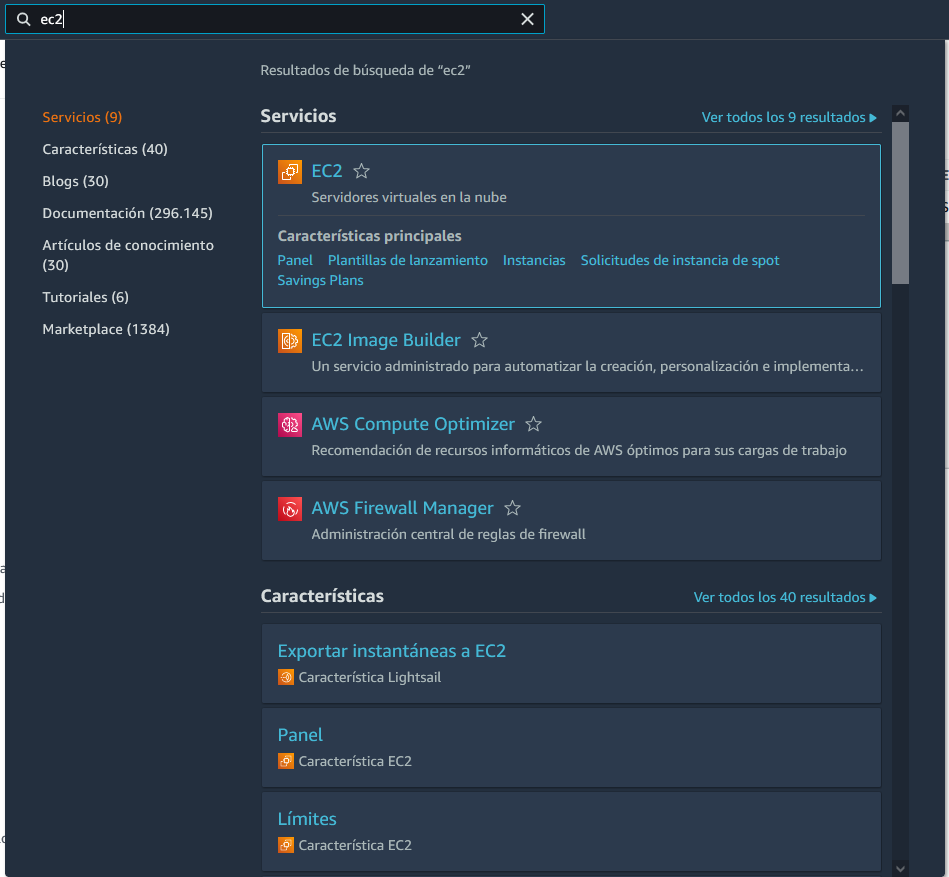
\includegraphics[width=1\textwidth]{figuras/paso1-ec2.png}
\caption{Resultado de introducir "EC2" en la barra de búsqueda de servicios de AWS.} 
\end{center}
\end{figure}

\begin{figure}[htb] 
\begin{center}
\label{fig:paso2-ec2}
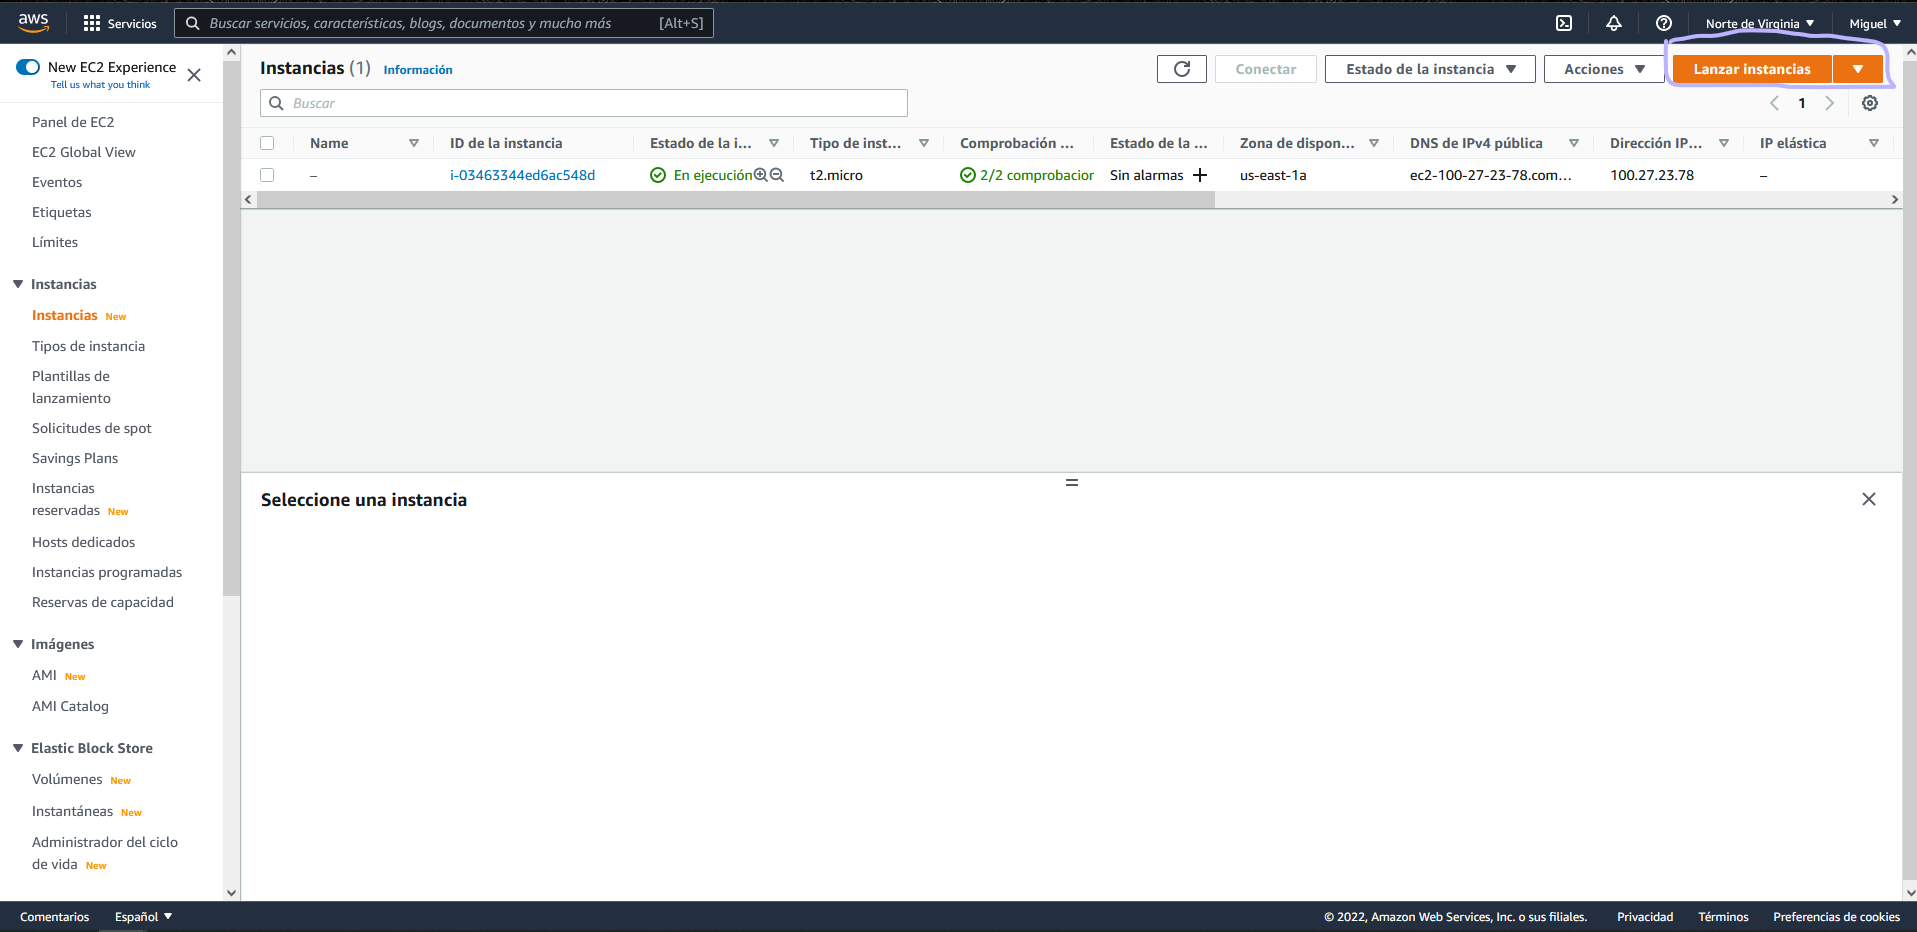
\includegraphics[width=1\textwidth]{figuras/paso2-ec2.png}
\caption{Panel de control del servicio EC2.} 
\end{center}
\end{figure}

\begin{figure}[htb] 
\begin{center}
\label{fig:paso3-ec2}
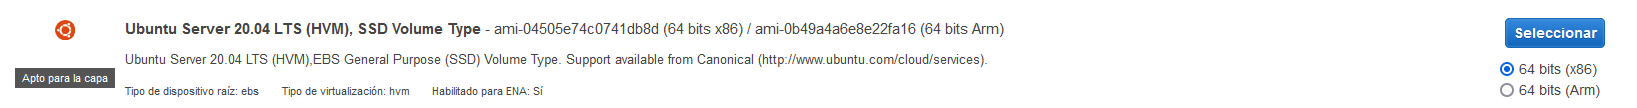
\includegraphics[width=1\textwidth]{figuras/paso3-ec2.png}
\caption{Imagen base a cargar en la instancia.} 
\end{center}
\end{figure}

\begin{figure}[htb] 
\begin{center}
\label{fig:paso4-ec2}
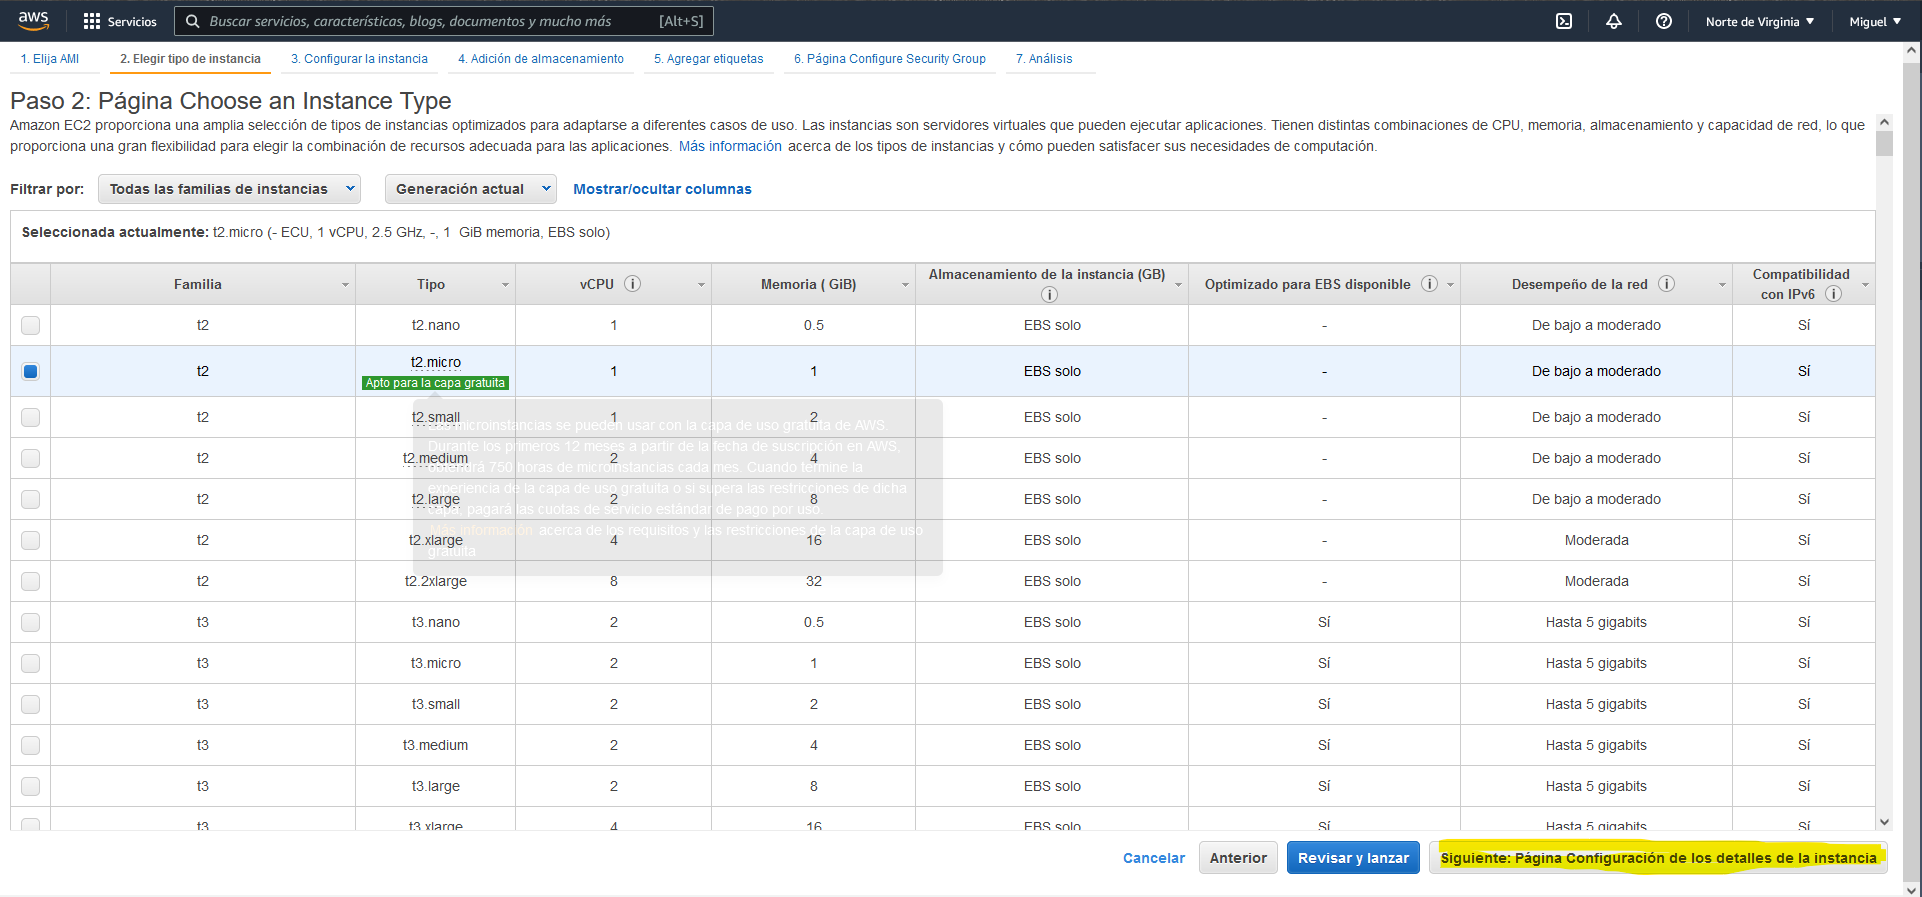
\includegraphics[width=1\textwidth]{figuras/paso4-ec2.png}
\caption{Página de selección de tipo de instancia.} 
\end{center}
\end{figure}

\begin{figure}[htb] 
\begin{center}
\label{fig:paso5-ec2}
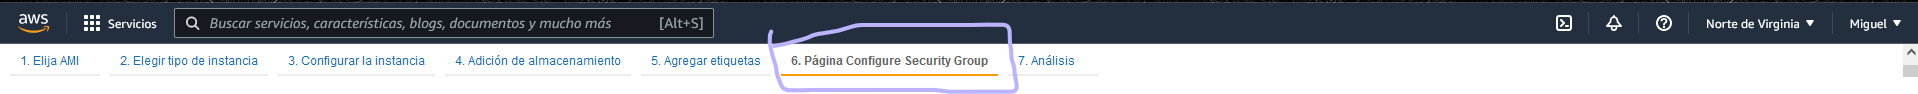
\includegraphics[width=1\textwidth]{figuras/paso5-ec2.png}
\caption{Selector de pasos para el despliegue de la instancia.} 
\end{center}
\end{figure}

\begin{figure}[htb] 
\begin{center}
\label{fig:paso6-ec2}
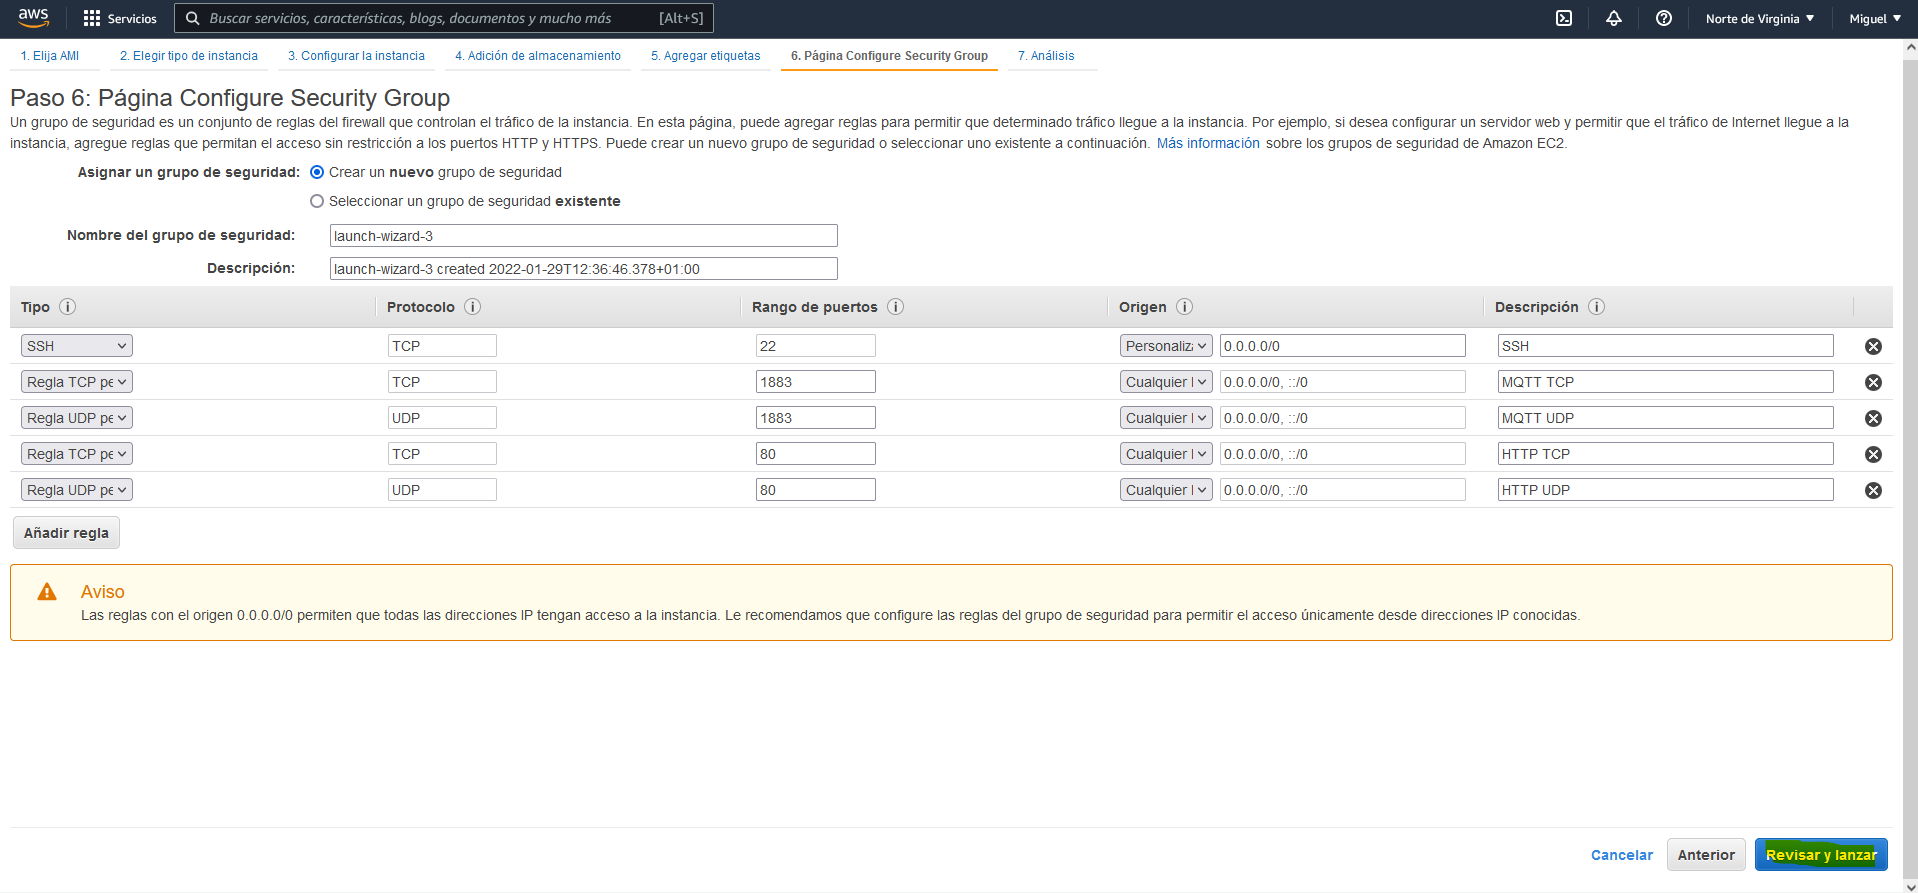
\includegraphics[width=1\textwidth]{figuras/paso6-ec2.png}
\caption{Página para configurar las políticas de seguridad con todos los puertos necesarios ya introducidos.} 
\end{center}
\end{figure}

\begin{figure}[htb] 
\begin{center}
\label{fig:paso7-ec2}
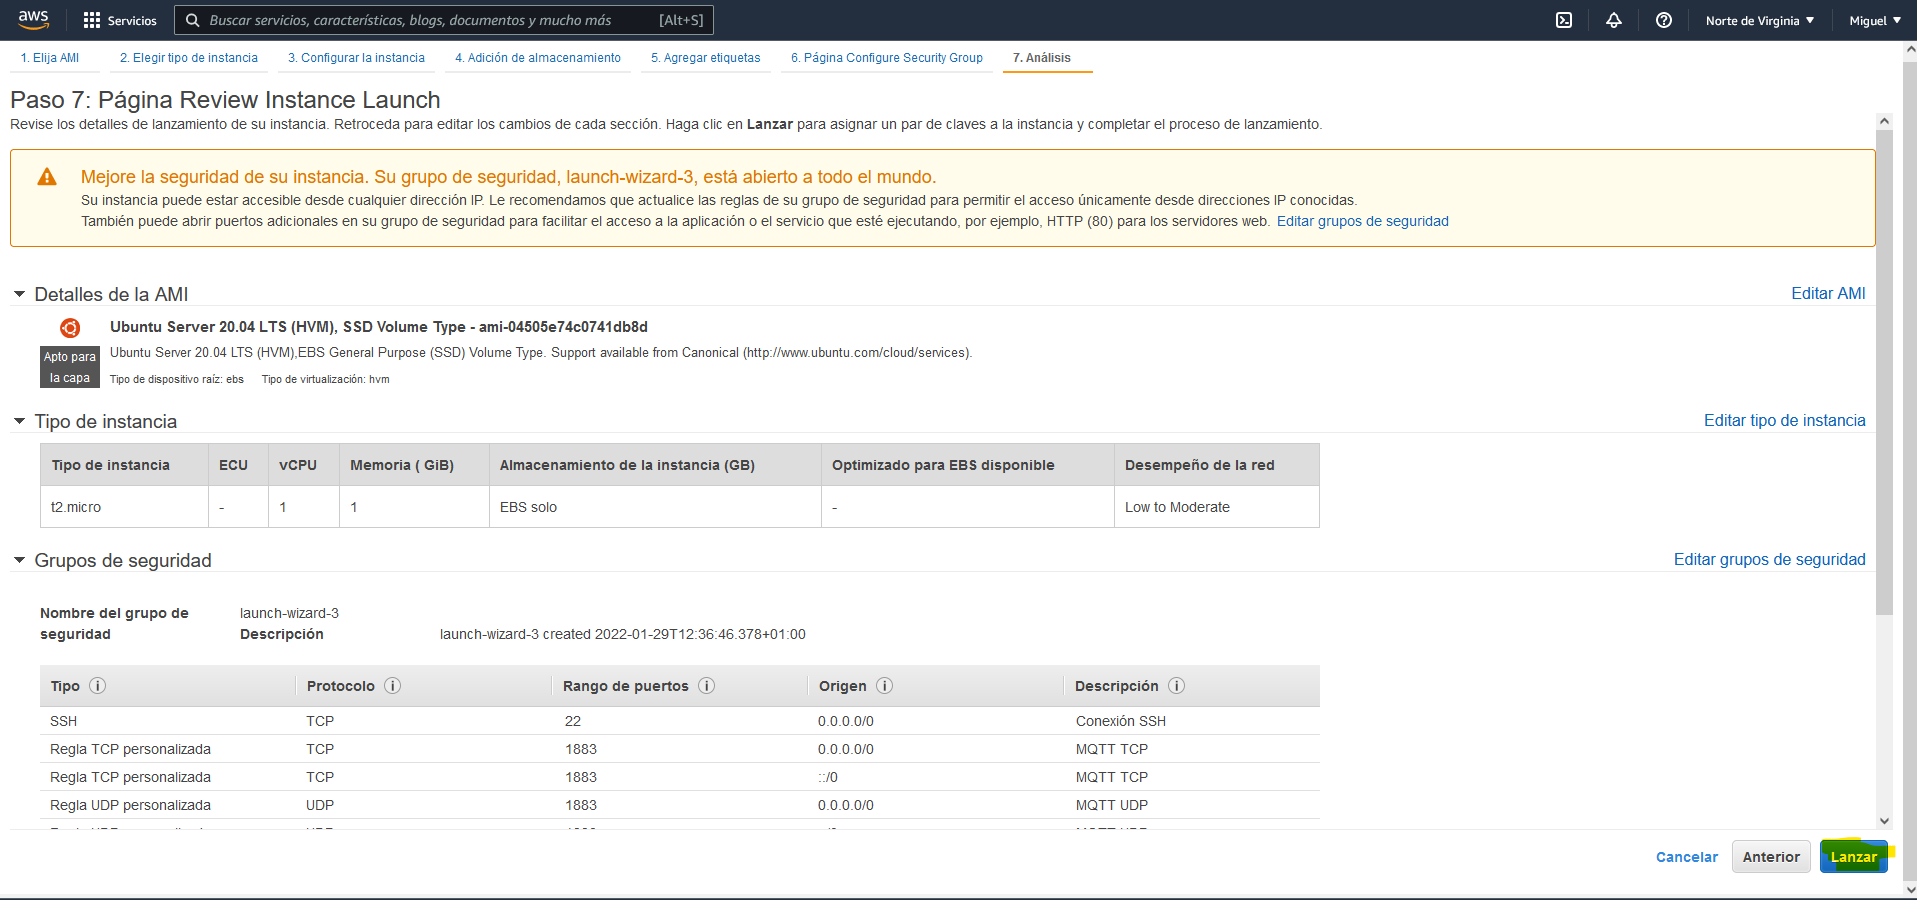
\includegraphics[width=1\textwidth]{figuras/paso7-ec2.png}
\caption{Página de revisión de la instancia antes del lanzamiento.} 
\end{center}
\end{figure}

\begin{figure}[htb]  
\begin{center}
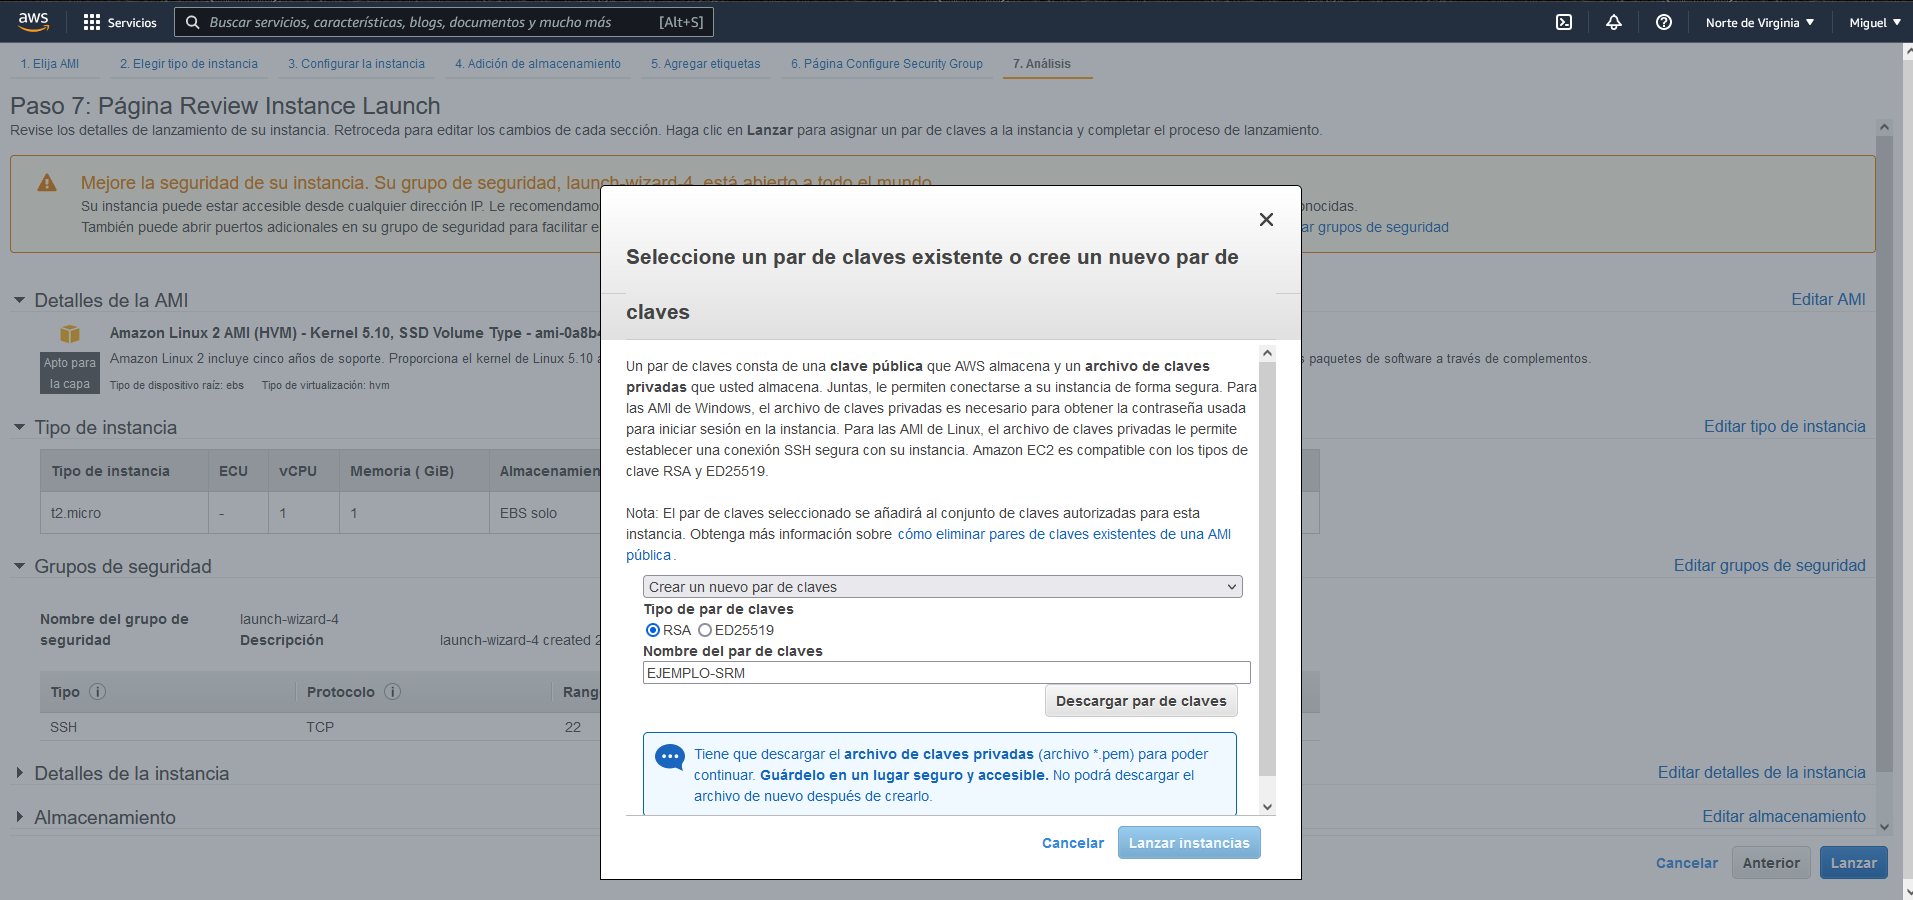
\includegraphics[width=1\textwidth]{figuras/paso10-ec2.png}
\caption{Aviso de creación del par de claves para la conexión SSH.} 
\label{fig:paso10-ec2}
\end{center}
\end{figure}

Una vez se ha completado esta lista de pasos, la instancia se ha creado de forma satisfactoria y debería estar en ejecución. Esto se puede comprobar desde el panel de control "EC2" que mostrará la instancia como "running" o "en ejecución" (es posible que si no aparece en este estado todavía esté iniciándose).

Para conectarse a la instancia se puede hacer desde el mismo panel de control realizando click derecho sobre la instancia y pulsando en "conectar". Luego seleccionando "Conexión de instancia EC2 (conexión SSH basada en navegador)" (figura \ref{fig:paso8-ec2}). Dejar el nombre de usuario por defecto y click en "Conectar". Se debería abrir una ventana nueva que funciona como terminal SSH.

\section{Instalación del servidor mosquitto}
Una vez realizada la conexión (no necesariamente desde el portal web, también se puede usar un cliente SSH convencional) ejecutar los siguiente comandos en la terminal.

\begin{enumerate}
    \item sudo apt-get update
    \item sudo apt-get install mosquitto
\end{enumerate}

Tras estos pasos, el servidor mosquitto debería estar instalado y se podría acceder a él desde cualquier host remoto mediante la IP pública (o el nombre del host público que ofrece AWS) en el puerto 1883. Para comprobar que el servidor está correctamente en funcionamiento se puede ejecutar el siguiente comando:

\begin{verbatim}
    ps -aux  | grep "/usr/sbin/mosquitto"
\end{verbatim}

Se deberían ver unas líneas con información referente al proceso del servidor mosquitto (figura \ref{fig:paso9-ec2}).

\begin{figure}[htb]  
\begin{center}
\label{fig:paso8-ec2}
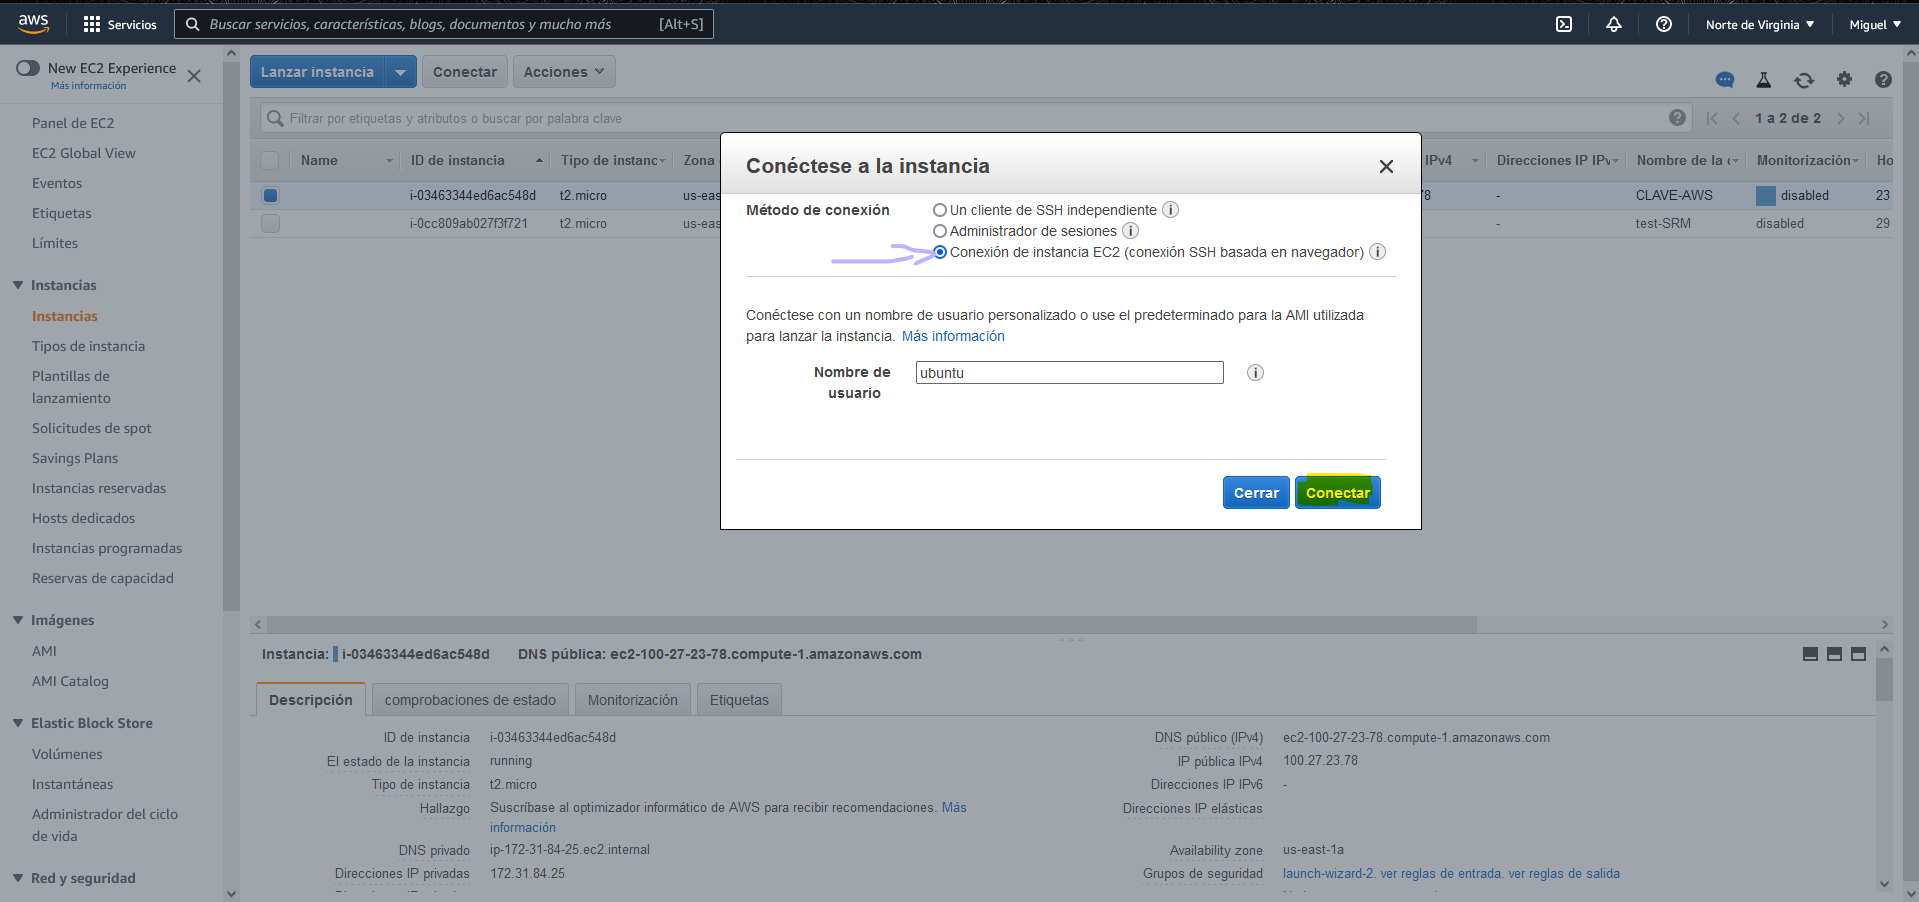
\includegraphics[width=1\textwidth]{figuras/paso8-ec2.png}
\caption{Conectarse a la instancia mediante SSH Web.} 
\end{center}
\end{figure}

\begin{figure}[htb]  
\begin{center}
\label{fig:paso9-ec2}
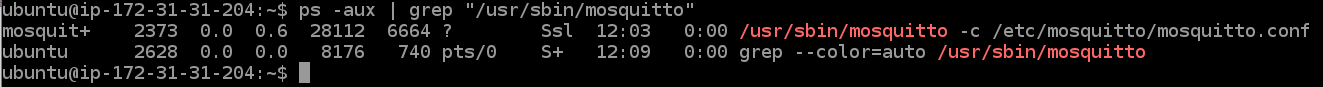
\includegraphics[width=1\textwidth]{figuras/paso9-ec2.png}
\caption{Ejemplo salida orden "ps -aux".} 
\end{center}
\end{figure}
\section{Inicio de la interfaz MQTT-REST}
Para poder ejecutar la interfaz MQTT-REST es necesario transferir el fichero al servidor. Es recomendable realizarlo mediante "scp" ya que utiliza una conexión SSH para realizarlo, pero cualquier otro medio es válido.

Una vez el fichero de la interfaz Python esté en la instancia debemos ejecutar las siguientes ordenes:

\begin{enumerate}
    \item sudo apt-get install python-is-python3
    \item sudo apt-get install pip
    \item pip install requests
    \item pip install paho-mqtt
\end{enumerate}

Tras instalar las dependencias, se puede proceder a lanzar la interfaz. Pero no sin antes modificar el servidor al que se debe conectar, que debe de ser la propia máquina virtual, para ello en la variable "MQTT\_SERVER" del programa, deberá modificarse a la IP (o el nombre del host) de la instancia creada (se puede obtener desde el panel de control EC2, seleccionando la instancia).

Para lanzar la intefaz hay que ejecutar los siguientes comandos (se supone que el fichero se denomina "main.py", se puede simplemente sustituir por el nombre del fichero si se ha modifcado):

\begin{enumerate}
    \item tmux
    \item python main.py
\end{enumerate}

Para abandonar la sesión de "tmux" sin detener la ejecución del \textit{script} hay que realizar la combinación "ctrl+B" y tras ello pulsar la tecla "D". "Tmux" es una utilidad que permite multiplexar terminales, en este caso lo utilizamos para dejar funcionando la interfaz en segundo plano sin terminar el proceso.

\section{Supervisor del servidor mosquitto}
Como la instancia gratuita no es muy fiable, se ha creado un pequeño \textit{script} capaz de detectar cuando el servidor MQTT no está en ejecución y poder reiniciarlo de forma automática. Este \textit{script} se puede ver en el anexo \ref{anexo:supervisor-mqtt}. Para poder ejecutarlo es necesario guardar el \textit{script} en un fichero ".sh", suponemos que el fichero se llama "mosquitto\_restart.sh".

Los pasos necesarios para que este \textit{script} se ejecute de forma periódica son:

\begin{enumerate}
    \item Ejectuar el comando "chmod +x mosquitto\_restart.sh"
    \item Ejecutar el comando "sudo -i"
    \item Ejecutar el comando "crontab -e"
    \item Pegar la siguiente línea "*/5 * * * * /home/ubuntu/mosquitto\_restart.sh" y guardar los cambios. Tras ello se puede cerrar el editor.
\end{enumerate}

Tras estos pasos, el \textit{script} se ejecutará cada 5 minutos y comprobará el estado del servidor mosquitto. Si no lo encuentra activo (existe solo una aparición al realizar la orden "ps", lo intentará volver a ejecutar.

\chapter{Conclusiones}
\label{cap:conclusiones}
A continuación se comentan las principales ideas que se extraen de este trabajo. Para ello, se comprueba si se han cumplido los objetivos propuestos en \ref{cap:objetivos}. Finalmente se concluye con posibles ampliaciones a realizar sobre este trabajo de cara a futuros trabajos.

\section{Objetivos alcanzados}
En esta sección se expondrán de nuevo los objetivos que se plantearon en \ref{cap:objetivos}, en base a estos, se comenta si se han llevado a cabo o no de forma satisfactoria junto con una breve explicación.

\begin{itemize}
    \item Definir una arquitectura de la comunicación. Esta parte se ha completado como una fase previa a la implementación de la IMR con tal de facilitar la implementación de esta misma y, por lo tanto, se considera que se ha completado de forma satisfactoria.
    \item Realizar la implementación del programa Python. Como se puede ver en el anexo \ref{anexo:codigo_interfaz}, este objetivo se ha cumplido. Además, también se provee una pequeña guía de usuario, asi como los detalles más relevantes de la implementación.
    \item Desplegar la aplicación y el servidor en el proveedor \textit{cloud}. Se ha hecho un pequeño tutorial sobre los pasos necesarios con tal de realizar el despliegue \textit{cloud}. También se ha presentado la dirección del host con tal de poder realizar pruebas (es recomendable utilizar MQTT-Explorer, de esta forma no es necesario realizar una aplicación de pruebas). Por todo lo mencionado anteriormente, se cree que este objetivo también ha sido alcanzado.
    \item Realizar un contenedor <<Docker>> para facilitar el despliegue.
\end{itemize}

\section{Trabajo futuro}

En esta sección se indican algunos posibles puntos de mejora o extensiones que se pueden realizar sobre el código ya desarrollado con tal de ofrecer una mejor calidad de servicio. Algunas posibles mejoras son (sin ningún orden en particular):

\begin{itemize}
    \item Establecer alguna forma de evitar que dos clientes diferentes puedan utilizar el mismo \textit{topic} para realizar las peticiones.
    \item Mejorar el conteo de las peticiones realizadas a la API con tal de maximizar el uso del nivel gratuito de la API de Open Weather Maps.
    \item Ofrecer soporte a varios hilos en la aplicación con tal de poder ofrecer servicio a más clientes al mismo tiempo.
    \item Implementar cierto nivel de reconfiguración en caso de fallo otra IMR pueda seguir ofreciendo servicio
    \item Definir reglas en el proveedor \textit{cloud} con tal de realizar un despliegue escalable que se adapte a la carga.
\end{itemize}

\chapter{ANEXO: Código Python para la interfaz}
\label{anexo:codigo_interfaz}
{\scriptsize
\begin{minted}[linenos]{python}
import requests
import json
import paho.mqtt.client as mqtt
import time

HELP_TEXT = '''Look at shorturl.at/akyES for some docs!'''

APIKEY = '8112c86d6d4fca7a4ab5fed299a7d259'
MQTT_SERVER = 'ec2-100-27-23-78.compute-1.amazonaws.com'
MQTT_PORT = 1883

API_PARAM={'appid':APIKEY}
WEATHER_ENDPOINT = 'https://api.openweathermap.org/data/2.5/weather'
AIR_POLLUTION_ENDPOINT = 'http://api.openweathermap.org/data/2.5/air_pollution' # Solo funciona por coordenadas
GEOCODING_ENDPOINT = 'http://api.openweathermap.org/geo/1.0/' # (Ciudad, estado de EEUU y codigo de pais, separados por coma Y [numero de localizaciones máx. 5]) o (codigo postal y codigo de pais)
ONECALL_ENDPOINT = 'https://api.openweathermap.org/data/2.5/onecall'
LAST_ONETIME_SENT = int(time.time()) # segs desde desde 1/1/1970 00:00:00
LAST_MIN_NORMAL_CHECK = int(time.time() / 60) # mins desde 1/1/1970 00:00:00
MADE_NORMAL_CALLS = 0

client = mqtt.Client(client_id="WeatherAPIID", 
                     clean_session=True,
                     userdata=None, 
                     protocol=mqtt.MQTTv311, 
                     transport="tcp")

def pushMsg(topic, payload):
    res = {"res": str(payload)}
    client.publish(topic, json.dumps(res),
                   qos=0, retain=False)

def on_connect(client, userdata, flags, rc):
    print("Connected to ", client._host, "port: ", client._port)
    print("Flags: ", flags, "returned code: ", rc)

    client.subscribe("reqs/+", qos=0)
    client.subscribe("help", qos=0)

def makeCurrentWeatherCall(msg, topic):

    params = dict(API_PARAM)
    reqtype = msg["type"]

    global MADE_NORMAL_CALLS

    try:
        resmode = msg["mode"]

        if (resmode != "JSON" and resmode != "xml" and resmode != "html"):
            pushMsg(topic+"/resp", "mode not one of JSON, XML or HTML")
            return
    except:
        resmode = "JSON"

    params["mode"]=resmode

    try:
        resunits = msg["units"]

        if (resunits != "standard" and resunits != "metric" and resunits != "imperial"):
            pushMsg(topic+"/resp", "units not one of standard, metric or imperial")
            return
    except:
        resunits = "standard"

    params["units"]=resunits

    try:
        reslang = msg["lang"]
    except:
        reslang = "en"

    params["lang"]=reslang

    if (reqtype == "city"):

        try:
            cityname_param = msg["city_name"]
            try:
                statecode = msg["state_code"]
                cityname_param = cityname_param + "," + statecode
                try:
                    countrycode = msg["country_code"]
                    cityname_param = cityname_param + "," + countrycode
                    print("City name AND state_code AND county_code")
                except:
                    print("City name AND state_code")
            except:
                print("Only city name")
        except:
            pushMsg(topic+"/resp", "At least 'city_name' must be present for a City name request")
            return

        params["q"]=cityname_param
        respuesta = requests.get(WEATHER_ENDPOINT, params=params)

        print(respuesta.content)
        pushMsg(topic+"/resp",respuesta.content)     
    elif (reqtype == "id"):
        try:
            params["id"] = msg["city_id"]
        except:
            pushMsg(topic+"/resp", "'city_id' needed for a city ID request")
            return

        respuesta = requests.get(WEATHER_ENDPOINT, params=params)

        print(respuesta.content)
        print(respuesta.url)
        pushMsg(topic+"/resp",respuesta.content)
    elif (reqtype == "geo"):
        try:
            params["lat"] = msg["lat"]
            params["lon"] = msg["lon"]
        except:
            pushMsg(topic+"/resp", "'lat' AND 'lon' must be present for a geo coord request")
            return
            
        respuesta = requests.get(WEATHER_ENDPOINT, params=params)

        print(respuesta.content)
        print(respuesta.url)
        pushMsg(topic+"/resp",respuesta.content)
    elif (reqtype == "zip"):
        zipparam = None
        try:
            zipparam = msg["zip"]
        except:
            pushMsg(topic+"/resp", "'zip' code must be present for a zip code request")
            return

        try:
            countrycode = msg["country_code"]
            zipparam = zipparam + "," + countrycode
        except:
            pushMsg(topic+"/resp", "'countrycode' code must be present for a zip code request")
            return
            
        params['zip']=zipparam
        respuesta = requests.get(WEATHER_ENDPOINT, params=params)

        print(respuesta.content)
        print(respuesta.url)
        pushMsg(topic+"/resp",respuesta.content)
    else:
        pushMsg(topic+"/resp","The selected request type is not valid for a current weather request")
        return
    
    MADE_NORMAL_CALLS += 1

def makeAirPollutionCall(msg, topic):
    
    global MADE_NORMAL_CALLS
    
    params = dict(API_PARAM)
    reqtype = msg["type"]

    if (reqtype == "current"):
        try:
            params["lat"] = msg["lat"]
            params["lon"] = msg["lon"]
        except:
            pushMsg(topic+"/resp", "'lat' AND 'lon' must be present for an Air Pollution Request")
            return
            
        respuesta = requests.get(AIR_POLLUTION_ENDPOINT, params=params)

        print(respuesta.content)
        print(respuesta.url)
        pushMsg(topic+"/resp",respuesta.content)
    elif (reqtype == "forecast"):
        try:
            params["lat"] = msg["lat"]
            params["lon"] = msg["lon"]
        except:
            pushMsg(topic+"/resp", "'lat' AND 'lon' must be present for an Air Pollution Forecast Request")
            return
            
        respuesta = requests.get(AIR_POLLUTION_ENDPOINT+"/forecast", params=params)

        print(respuesta.content)
        print(respuesta.url)
        pushMsg(topic+"/resp",respuesta.content)
    elif (reqtype == "history"):
        try:
            params["lat"] = msg["lat"]
            params["lon"] = msg["lon"]
        except:
            pushMsg(topic+"/resp", "'lat' AND 'lon' must be present for an Air Pollution Historical Request")
            return
        
        try:
            params["start"] = int(msg["start"])
            params["end"] = int(msg["end"])
        except:
            pushMsg(topic+"/resp", "'start' AND 'end' must be present AND an integer for an Air Pollution Historical Request")
            return
        
        respuesta = requests.get(AIR_POLLUTION_ENDPOINT+"/history", params=params)

        print(respuesta.content)
        print(respuesta.url)
        pushMsg(topic+"/resp",respuesta.content)
    else:
        pushMsg(topic+"/resp","The selected request type is not valid for an Air pollution request")
        return

    MADE_NORMAL_CALLS += 1

def makeGeocodingCall(msg, topic):

    global MADE_NORMAL_CALLS

    params = dict(API_PARAM)
    reqtype = msg["type"]
    limit = 1
    try:
        limit = msg["limit"]
    except:
        print("Can't parse the limit parameter, setting a 1 default")

    if (reqtype == "reverse"):
        try:
            params["lat"] = msg["lat"]
            params["lon"] = msg["lon"]
        except:
            pushMsg(topic+"/resp", "'lat' AND 'lon' must be present for a Reverse Geocoding Request")
            return
        
        params["limit"] = limit
        respuesta = requests.get(GEOCODING_ENDPOINT+"reverse", params=params)

        print(respuesta.content)
        print(respuesta.url)
        pushMsg(topic+"/resp",respuesta.content)
    elif (reqtype == "direct_name"):
        try:
            cityname_param = msg["city_name"]
            try:
                statecode = msg["state_code"]
                cityname_param = cityname_param + "," + statecode
                try:
                    countrycode = msg["country_code"]
                    cityname_param = cityname_param + "," + countrycode
                    print("City name AND state_code AND county_code")
                except:
                    print("City name AND state_code")
            except:
                print("Only city name")
        except:
            pushMsg(topic+"/resp", "At least 'city_name' must be present for a Direct Geocoding Name Request")
            return

        params["q"]=cityname_param
        params["limit"] = limit
        respuesta = requests.get(GEOCODING_ENDPOINT+"/direct", params=params)

        print(respuesta.content)
        print(respuesta.url)
        pushMsg(topic+"/resp",respuesta.content)
    elif (reqtype == "direct_zip"):
        zipparam = None
        try:
            zipparam = msg["zip"]
        except:
            pushMsg(topic+"/resp", "'zip' code must be present for a zip code request")
            return

        try:
            countrycode = msg["country_code"]
            zipparam = zipparam + "," + countrycode
        except:
            pushMsg(topic+"/resp", "'countrycode' code must be present for a zip code request")
            
        params['zip']=zipparam
        respuesta = requests.get(GEOCODING_ENDPOINT+"/zip", params=params)

        print(respuesta.content)
        print(respuesta.url)
        pushMsg(topic+"/resp",respuesta.content)
    else:
        pushMsg(topic+"/resp","The selected request type is not valid for an Air pollution request")
        return

    MADE_NORMAL_CALLS += 1

def makeOneTimeCall(msg, topic):

    global LAST_ONETIME_SENT

    params = dict(API_PARAM)
    reqtype = msg["type"]

    try:
        resunits = msg["units"]

        if (resunits != "standard" and resunits != "metric" and resunits != "imperial"):
            pushMsg(topic+"/resp", "units not one of standard, metric or imperial")
            return
    except:
        resunits = "standard"

    params["units"]=resunits

    try:
        reslang = msg["lang"]
    except:
        reslang = "en"

    params["lang"]=reslang

    if(reqtype == 'non_historical'):
        try:
            params["lat"] = msg["lat"]
            params["lon"] = msg["lon"]
        except:
            pushMsg(topic+"/resp", "'lat' AND 'lon' must be present for a One Call request")
            return

        to_exclude = None
        try:
            string_list = msg['exclude']
            excluded_list = list(dict.fromkeys(string_list.split(',')))
            to_exclude = ','.join(excluded_list)
            params['exclude']=to_exclude
        except:
            print("No hay excluidos, o no se han podido interpretar bien")

        respuesta = requests.get(ONECALL_ENDPOINT, params=params)

        print(respuesta.content)
        print(respuesta.url)
        pushMsg(topic+"/resp",respuesta.content)
    elif (reqtype == 'historical'):
        try:
            params["lat"] = msg["lat"]
            params["lon"] = msg["lon"]
        except:
            pushMsg(topic+"/resp", "'lat' AND 'lon' must be present for a One Call request")
            return

        try:
            params["dt"] = msg["dt"]
            currSecs = int(time.time())

            if ((currSecs - int(params["dt"])) > 432000):
                pushMsg(topic+"/resp", "'dt' must be from the last 5 days")
                return
        except:
            pushMsg(topic+"/resp", "'dt' must be present for a One Call request ")
            return

        to_exclude = None
        try:
            string_list = msg['exclude']
            excluded_list = list(dict.fromkeys(string_list.split(',')))
            to_exclude = ','.join(excluded_list)
            params['exclude']=to_exclude
        except:
            print("No hay excluidos, o no se han podido interpretar bien")

        respuesta = requests.get(ONECALL_ENDPOINT+"/timemachine", params=params)

        print(respuesta.content)
        print(respuesta.url)
        pushMsg(topic+"/resp",respuesta.content)

    else:
        pushMsg(topic+"/resp","The selected request type is not valid for a One Call Request")
        return
    
    LAST_ONETIME_SENT = int(time.time())

def unrecognizedCall(topic):
    pushMsg(topic+"/resp", HELP_TEXT)


def parse_req(msg):
    try:
        themsg = json.loads(msg.payload.decode("utf-8"))
    except:
        pushMsg(msg.topic+"/resp", "Could not parse JSON request, check the payload, then, try again!")

    currTime = int(time.time())
    CallType = themsg["CallType"]

    global LAST_MIN_NORMAL_CHECK
    global LAST_ONETIME_SENT
    global MADE_NORMAL_CALLS

    if(CallType == "CurrentWeather"):        
        if(int(currTime / 60) > LAST_MIN_NORMAL_CHECK):
            MADE_NORMAL_CALLS = 0
            LAST_MIN_NORMAL_CHECK = currTime / 60

        if(MADE_NORMAL_CALLS < 23):
            makeCurrentWeatherCall(themsg, msg.topic)      # 23 CALLS / MIN
        else:
            pushMsg(msg.topic + "/resp","API CALLS LIMIT REACHED FOR THIS MINUTE. TRY AGAIN LATER!")
    elif (CallType == "OneTime"):

        if((currTime - LAST_ONETIME_SENT) >= 90):
            makeOneTimeCall(themsg, msg.topic)   # OneTime APROX 1 EVERY 1.5 MIN
        else:
            pushMsg(msg.topic + "/resp","ONETIME API CALL LIMIT REACHED THIS 90 s PERIOD. TRY AGAIN LATER!")
    elif (CallType == "AirPollution"):
        if(int(currTime / 60) > LAST_MIN_NORMAL_CHECK):
            MADE_NORMAL_CALLS = 0
            LAST_MIN_NORMAL_CHECK = currTime / 60

        if(MADE_NORMAL_CALLS < 23):
            makeAirPollutionCall(themsg, msg.topic)        # 23 CALLS / MIN
        else:
            pushMsg(msg.topic + "/resp","API CALLS LIMIT REACHED FOR THIS MINUTE. TRY AGAIN LATER!")
    elif (CallType == "Geocoding"):
        if(int(currTime / 60) > LAST_MIN_NORMAL_CHECK):
            MADE_NORMAL_CALLS = 0
            LAST_MIN_NORMAL_CHECK = currTime / 60

        if(MADE_NORMAL_CALLS < 23):
            makeGeocodingCall(themsg, msg.topic)           # 23 CALLS / MIN
        else:
            pushMsg(msg.topic + "/resp","API CALLS LIMIT REACHED FOR THIS MINUTE. TRY AGAIN LATER!")
    else:
        unrecognizedCall(msg.topic)

def public_help_message():
    pushMsg("help", HELP_TEXT)


def on_message(client, userdata, msg):
    if (msg.topic == "help"):
        public_help_message()
    else:
        parse_req(msg)
    
client.on_connect = on_connect
client.on_message = on_message
client.username_pw_set("WeatherAPIID", password=None)
client.connect(MQTT_SERVER, port=MQTT_PORT, keepalive=60)
client.loop_forever()
\end{minted}
}

\chapter{ANEXO: Documentación Interfaz MQTT-REST}
\label{anexo:IMR-docs}
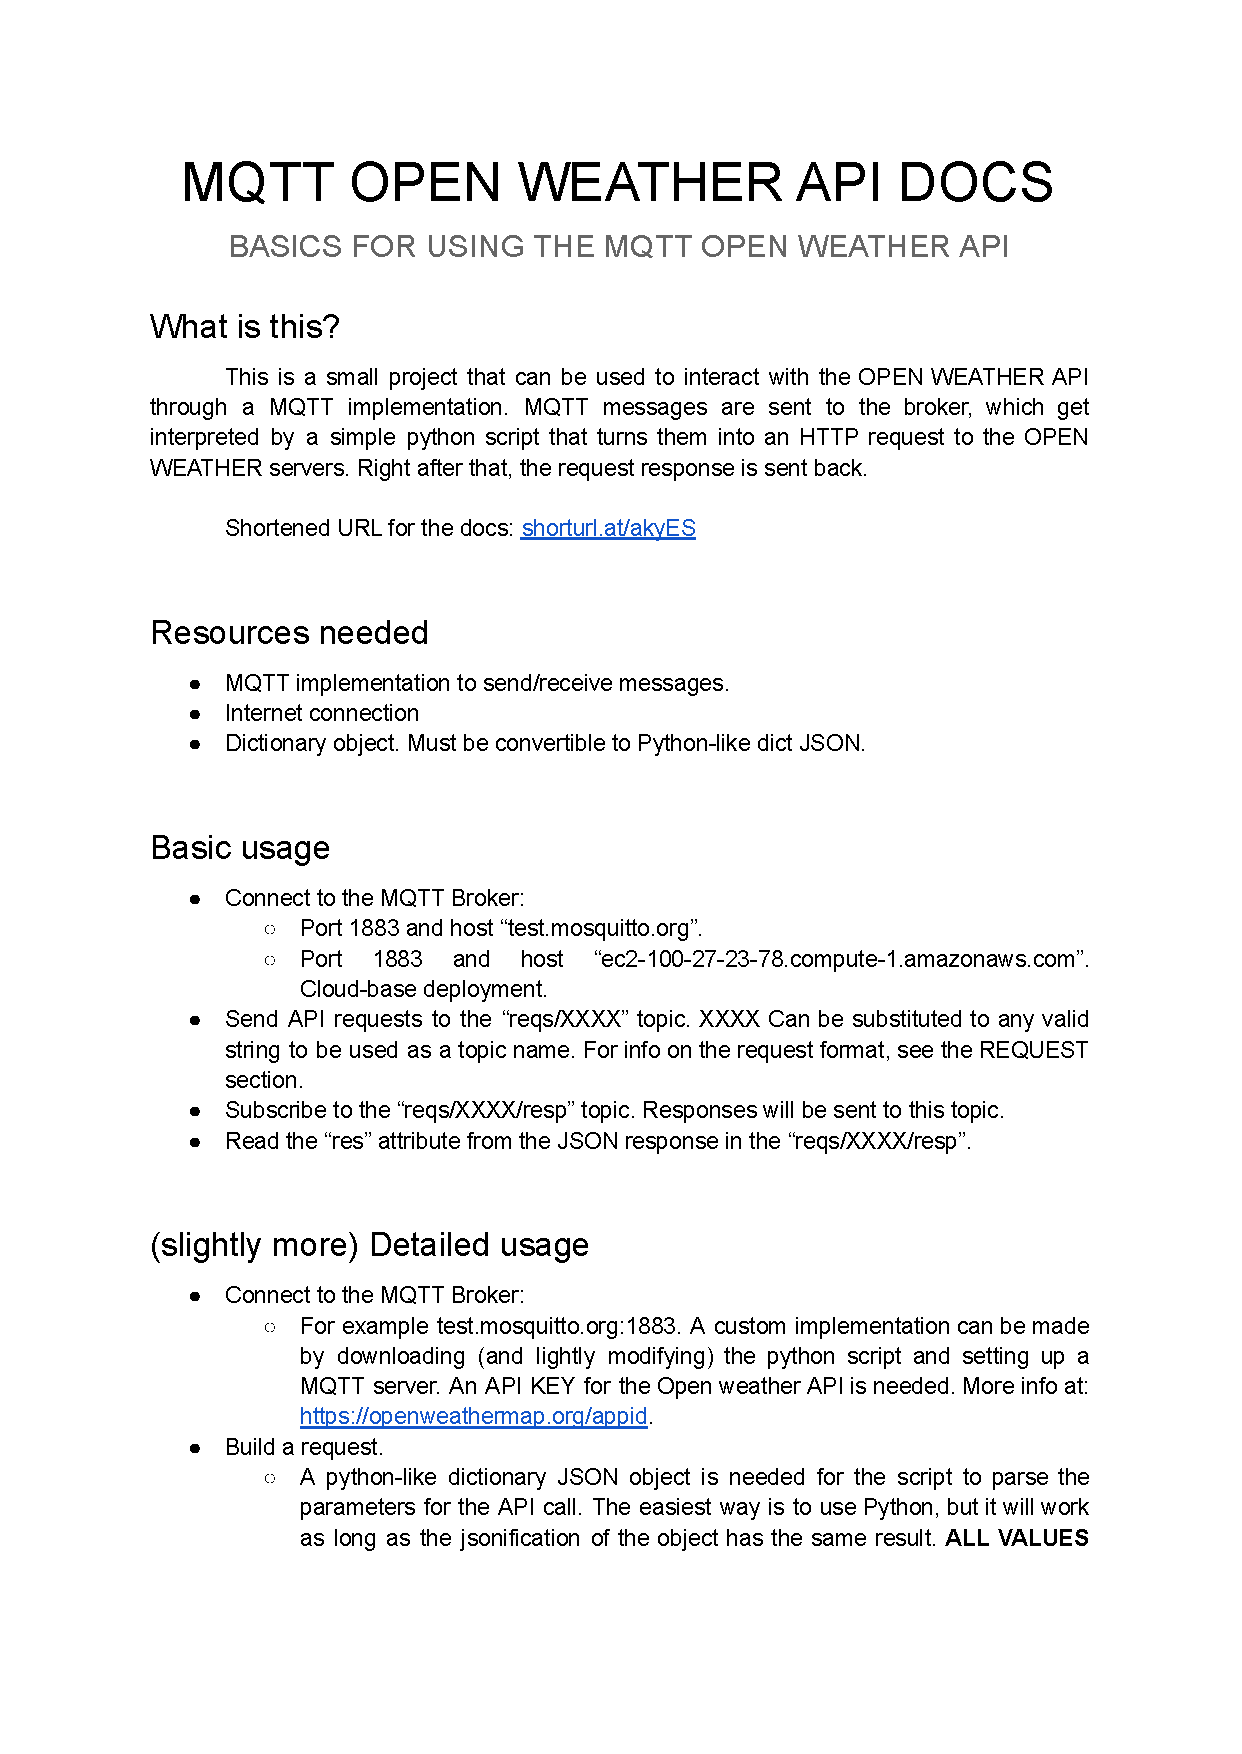
\includepdf[pages=-,pagecommand={},width=\textwidth]{figuras/IMR-docs.pdf}
\chapter{ANEXO: Script supervisor del servidor mosquitto}
\label{anexo:supervisor-mqtt}
\begin{minted}{bash}
if [ "`ps -aux | grep /usr/sbin/mosquitto | wc -l`" == "1" ]
then

        echo "mosquitto wasnt running so attempting restart" >> /home/ubuntu/cron.log
        systemctl restart mosquitto
        exit 0

fi
echo "$SERVICE is currently running" >> /home/ubuntu/cron.log
exit 0
\end{minted}
\end{document}